\documentclass[10pt,a4paper]{article}
\usepackage{blindtext}
\usepackage{subcaption}
\usepackage{graphicx}
\usepackage{tikz}
\usepackage{amssymb}
\usepackage{caption}
\usepackage{amsmath}
\usepackage{circuitikz}
\usepackage{hyperref}
\usepackage{amssymb}
\usepackage{amsmath}
\usepackage{listings}

\lstset{
    inputencoding=utf8,
    extendedchars=true,
    literate={á}{{\'a}}1 {é}{{\'e}}1 {í}{{\'i}}1 {ó}{{\'o}}1 {ú}{{\'u}}1 {ñ}{{\~n}}1 {Á}{{\'A}}1 {É}{{\'E}}1 {Í}{{\'I}}1 {Ó}{{\'O}}1 {Ú}{{\'U}}1 {Ñ}{{\~N}}1
}
\input{AEDmacros}
\newcommand{\notimplies}{\;\not\!\!\!\implies}
\title{Análisis II}
\author{Tomás Agustín Hernández}
\date{}

\begin{document}
\maketitle

\begin{figure}[b]
    \centering
    \begin{tikzpicture}[remember picture,overlay]
        \node[anchor=south east, inner sep=0pt, xshift=-1cm, yshift=2cm] at (current page.south east) {
            \begin{minipage}[b]{0.5\textwidth}
                \includegraphics[width=\linewidth]{logo_uba.jpg}
                \label{fig:bottom}
            \end{minipage}
        };
    \end{tikzpicture}
\end{figure}

\newpage
\section*{Dilatación}
Sean $a, n \in \float $ decimos que estamos dilatando al número a sí y solo sí $ a \ = \ a \ * \ n$ con $n >= 1$
\section*{Contracción}
Sean $a, n \in \float $ decimos que estamos contrayendo al número a sí y solo sí $ a \ = \ a \ * \ n$ con $ 0 > n < 1$
\section*{Plano Real $\float^{2}$}
Se define como $\float^{2} = \float x \float = \{(a, b): a, b \in \float\}$
Aquí, los puntos se definen con dos coordenadas: x e y.
\section*{Plano Real $\float^{3}$}
También conocido como $espacio$. \\
Se define como $\float^{3} = \float x \float = \{(a, b, c): a, b, c \in \float\}$
\subsection*{Orientación de los ejes}
Se rigen por la regla de la mano derecha. Cuando vamos girando, hacia donde queda apuntando el dedo es el eje z.
\section*{Distancia entre dos puntos}
Sean dos puntos $P = (a_{1}, a_{2}) \ y \ Q = (b_{1}, b_{2})$, definimos la distancia entre dos puntos como "la distancia entre P y Q es la raíz cuadrada de la suma de los cuadrados de las diferencias de sus coordenadas." \\ 
\[dist(P,Q) = \sqrt[]{(b_{2} - a_{2})^{2} + (b_{1} - a_{1})^{2}}\]
Esta misma definición es generalizable para n coordenadas. \\
\textbf{Nota}: $dist(P, Q) = long(\bar{PQ})$

\section*{Circunferencias y Discos (Solo en $\float^{2}$)}
\subsection*{Circunferencia}
Sea un centro $C_{0} = (a_{0}, b_{0})$ y radio $r > 0$ definimos a una circunferencia como: 
\[\{(x, y) \in \float^{2}: \sqrt[]{(x - a_{0})^{2} + (y - b_{0})^{2} \textcolor{purple}{=} r}\}\] 

Si notamos que la circunferencia está definida usando la definición de distancia entre dos puntos, si desarrollamos la ecuación de la circunferencia nos queda algo así: 
\[(x-x_{1})^{2} + (y-x_{2})^{2} = r^{2}\]

\textbf{Importante}: La circunferencia \$' =  $\{(x, y) \in \float^{2}: \sqrt[]{x^{2} + y^{2} = 1}\}$ es conocida como Circunferencia Unidad.
\subsection*{Disco Abierto}
Cada vez que leamos la palabra $abierto$ quiere decir que no incluye los bordes, sino solo el contenido.
Definimos el Disco Abierto de centro $C_{0}$ y radio $r > 0$ como 
\[\{(x, y) \in \float^{2}: \sqrt[]{(x - a_{0})^{2} + (y - b_{0})^{2} < r}\}\]

\subsection*{Disco Cerrado}
Exactamente igual que el Disco Abierto pero con los bordes incluidos. \\ 
Definimos el Disco Abierto de centro $C_{0}$ y radio $r > 0$ como 
\[\{(x, y) \in \float^{2}: \sqrt[]{(x - a_{0})^{2} + (y - b_{0})^{2} \textcolor{purple}{\le} r}\}\]
\section*{Esferas y Bolas (Solo en $\float^{3}$)}
\subsection*{Esfera}
Sea un centro $ C_{0} = (a_{0}, b_{0}, c_{0})$ y radio $r > 0$ definimos una esfera como: 
\[\{(x, y, z) \in \float^{3}: \sqrt[]{(x_{0} - a_{0})^{2} + (y_{0} - b_{0})^{2} + (z_{0} - c_{0})^{2} \textcolor{purple}{=} r}\}\]
\subsection*{Definición formal de Esfera}
\[ Br(P) = \{X = (x_{1}, ..., x_{n}) \in \float^{n} : ||X-P|| = r\}\]
\begin{center}
    \begin{minipage}[b]{0.3\textwidth}
        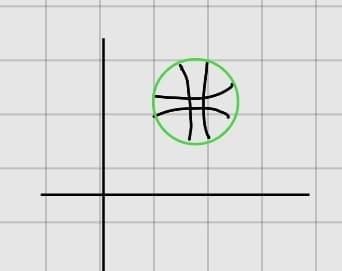
\includegraphics[width=\linewidth]{assets/esfera.jpg}
        \centering
        \label{fig:esfera}
    \end{minipage}
\end{center}
\subsection*{Bola Abierta}
Misma idea que Disco Abierto pero en $\float^{3}$
\[\{(x, y, z) \in \float^{3}: \sqrt[]{(x - a_{0})^{2} + (y - b_{0})^{2} + (z_{0} - c_{0})^{2} < r}\}\] 
\subsection*{Definición formal de Bola Abierta}
\[ Br(P) = \{X = (x_{1}, ..., x_{n}) \in \float^{n} : ||X-P|| < r\}\]
\begin{center}
    \begin{minipage}[b]{0.3\textwidth}
        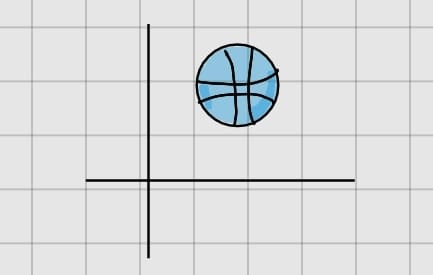
\includegraphics[width=\linewidth]{assets/bola_abierta.jpg}
        \centering
        \label{fig:bola_abierta}
    \end{minipage}
\end{center}
\subsection*{Bola Cerrada}
Misma idea que Disco Cerrado pero en $\float^{3}$
\[\{(x, y, z) \in \float^{3}: \sqrt[]{(x - a_{0})^{2} + (y - b_{0})^{2} + (z_{0} - c_{0})^{2} \ \textcolor{purple}{\le} \ r}\}\]
\textbf{Nota}: Véase $\hyperref[subsec:completar_cuadrados_esfera]{\underline{anexo}}$ para ver ejercicios de completar cuadrados y encontrar el centro y radio de una esfera.
\subsection*{Definición formal de Bola Cerrada}
\[ Br(P) = \{X = (x_{1}, ..., x_{n}) \in \float^{n} : ||X-P|| \le r\}\]
\begin{center}
    \begin{minipage}[b]{0.3\textwidth}
        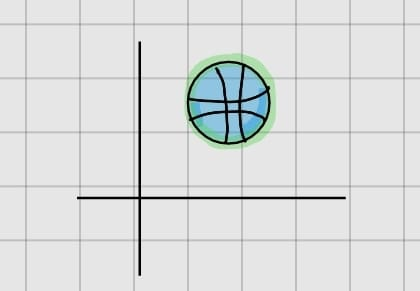
\includegraphics[width=\linewidth]{assets/bola_cerrada.jpg}
        \centering
        \label{fig:bola_cerrada}
    \end{minipage}
\end{center}
\section*{Aclaración sobre enunciados}
Importante siempre prestar atención a la dimensión donde trabajamos. \\
Es decir $x^{2} + y^{2} = 4$ puede representar dos cosas diferentes si estamos en $\float^{2}$ o en $\float^{3}$
\section*{Vectores}
Los vectores tienen dirección, sentido y longitud. \\
Sean dos puntos $P, Q \in \float^{n}$, definimos un vector $V \in \float^{n}$ como $ \bar{PQ} = Q - P$.
\subsection*{Vectores Equivalentes}
Dos vectores son equivalentes si tienen misma dirección, sentido y longitud. 
\subsection*{Vectores Iguales}
Dos vectores son iguales si son equivalentes y además parten del mismo punto.
\subsection*{Suma de Vectores}
Sean $ u, v $ vectores $\in \float^{n}$. La suma de ambos se realiza coordenada a coordenada.
$ u + v = (u_{1} + v_{1}, u_{2} + v_{2}, ..., u_{n} + v_{n})$
\subsection*{Producto por Escalar}
Sea $t \in \float$ y u un vector.
$ t * u = (tu_{1}, tu_{2}, ..., tu_{3})$
\subsection*{Regla del Paralelo}
Se utiliza para ver como queda la traslación del vector $u+v$ luego de sumar ambos vectores.
\subsection*{Propiedades de los vectores}
\begin{itemize}
    \item La suma es conmutativa: u + v = v + u
    \item Sea un valor $ t \in \float $, definimos la distributiva con vectores como t(u+v) = tu + tv
\end{itemize}
\subsection*{Norma de un Vector}
Definimos la norma de un vector como $ || V || = \sqrt[]{(v_{1})^{2} + (v_{2})^2 + ... + (v_{n})^2}$ 
\subsection*{Relación entre distancia entre dos puntos y la norma}
Es fácil notar que $ ||B-A|| = ||A-B||. $ 
Definimos la \textbf{equivalencia} de las siguientes fórmulas: 
\[ dist(A, B) = ||B-A|| \equiv ||A-B|| \]
\subsection*{Propiedades de la norma}
\begin{itemize}
    \item $||V||  \ge  0$
    \item $|V| = \sqrt[]{V^{2}}$
    \item $||V|| = dist(V, 0)$
    \item $\alpha \in \float, ||\alpha * V|| = ||\alpha|| * ||V||$: en criollo quiere decir que si multiplico un escalar dentro de la norma, es lo mismo que sacarlo hacia afuera y hacerlo por separado. 
    \item $||V+W|| \le ||V|| + ||W||$: desigualdad Triangular (DT)
    \item $||V-W|| \le ||V|| + ||-W||$: esto tiene sentido pues $||-w||$ es positivo. Entonces queda $||V-W|| \le ||V|| + ||W||$
    \begin{itemize}
        \item Importante: Esto se utiliza mucho para acotar. $ ||V+W||$ y $||V-W||$ se acotan por $ ||V|| + ||-W|$
    \end{itemize}
\end{itemize}
\textbf{Importante}: Si aplico la NORMA a un número, es como aplicar el módulo.
\section*{Producto Interno (Producto Escalar / Producto Punto)}
Sean $u, v \in \float^{n}$. Definimos el producto interno, como la multiplicación \textbf{coordenada a coordenada} de los vectores. \textbf{Siempre devuelve un número.} \\
Hay dos formas de notarlo
\[<u,v> = u * v\]
\subsection*{Vectores Perpendiculares}
Sean $u, v \in \float^{n}$. Si el producto escalar entre dos vectores es 0, entonces los vectores son perpendiculares.
\subsection*{Propiedades del Producto Interno}
\begin{itemize}
    \item $u * u = ||u||^{2}$
    \item Conmutatividad: $u * v = v * u$
    \item Distributividad: Sean $u, v, w \in \float^{n}$, entonces $(u+v) * w = uw + vw$ 
    \item $ t \in \float, (t * u) * v = t * (u * v) = u * (t * v)$
\end{itemize}
\textbf{Importante}: No se pueden multiplicar 3 vectores con el producto interno, porque el producto interno devuelve un NÚMERO. Si multiplico 3 vectores, sería multiplicar primero dos (devuelve un número) y según si es $ > 1 $ o no, estaríamos dilatando/contrayendo otro vector. 
\subsection*{Propiedad importante de la norma y el Producto Interno}
Sean $v, w \in \float^{n}$
\[ v * w = ||v|| * ||w| * cos(\theta)\] con $ 0 \le \theta \le \pi $
\subsection*{Teorema de Cauchy-Schwartz}
$\forall u, v \in \float^{n}$ vale $ |u * v| \le ||u|| * ||v||$
\textbf{Importante}: Si $|u * v| = ||u|| * ||v||$ entonces $ v // u$ (v es paralelo a u)
\section*{Proyecciones}
Sean $v, w \in \float^{n}$. Queremos calcular la proyección de w en la dirección de v. 
\[P_{v}(w) = w * \frac{v}{||w||} * \frac{v}{||v||} = w * v * \frac{v}{||v||^{2}} = \frac{w * v}{v * v} = \frac{w * v}{v^{2}} * v\]
\section*{Producto Vectorial / Cruz (Solo en $\float^{3}$)}
Sean $v, w \in \float^{3}$. Se utiliza para calcular un \textbf{vector perpendicular} a los dos que se nos envían.
\[
\begin{pmatrix}
\hat{i} & \hat{j} & \hat{k} \\
a & b & c\\
d & e & f
\end{pmatrix}
\]
Entonces, el cálculo que hay que hacer es: ((b * f) - (c * e), \textcolor{red}{-} ((a * f) - (c * d)), ((a * e) - (b * d)))
\textbf{Importante}: Si este cálculo da 0, entonces los vectores son paralelos.
\subsection*{Propiedades del Producto Vectorial}
\begin{itemize}
    \item (V x W) es perpendicular a V y W.
    \begin{itemize}
        \item Esto es re útil para cuando encontramos una normal para el plano y queremos ver si efectivamente es perpendicular a ambos vectores.
    \end{itemize}
    \item (W x V) = - (V x W): Es decir, no son iguales si los invertimos, si lo invierto le cambio el signo. 
\end{itemize}
\section*{Planos en $\float^{3}$}
Dado un \textbf{vector normal N} y un \textbf{punto de paso P} construimos la ecuación del plano $\pi$ que es perpendicular al \textbf{vector normal} y contiene al punto P (es decir, P verifica la ecuación del plano).
\subsection*{Hallar vector normal N de un Plano}
El vector normal N de un Plano lo podemos hallar comúmnente de las siguientres maneras 
\begin{itemize}
    \item Si tenemos 3 puntos, ABC podemos hacer la diferencia y generar 2 vectores directores. Es decir, AB y BC o AB y AC. Luego aplicamos el producto cruz y ya tenemos la normal al plano. Por último podemos tomar cualquier punto.
    \begin{itemize}
        \item Como tenemos la NORMAL tenemos (a, b, c) nos falta d. Para generar d podemos evaluar ax + by + cz con cualquier punto de paso. El número que da como resultado es d.
    \end{itemize}
\end{itemize}
\subsection*{Ecuación Paramétrica del Plano}
$ \pi: \lambda(x_{1}, x_{2}, x_{3}) + \gamma(y_{1}, y_{2}, y_{3}) + (p_{1}, p_{2}, p_{3})$
\subsection*{Ecuación Implícita del Plano}
$ \pi: ax + by + cz = d$
\subsection*{Saber si un punto está en un plano}
Debe verificar la ecuación implícita.
\section*{Rectas Paramétricas}
En $\float^{2} = L:(x,y) = \alpha (v_{1}, v_{2}) + (P_{1}, P_{2}), \alpha \in \float$ \\
En $\float^{3} = L:(x,y,z) = \alpha (v_{1}, v_{2}, v_{3}) + (P_{1}, P_{2}, P_{3}), \alpha \in \float$
\subsection*{Intersección entre dos rectas}
Sean $L_{1}, L_{2}$ dos rectas.
La intersección entre dos rectas se da en un punto específico. Por lo tanto, se espera que la intersección sea un número y además, este número pertenece a $L_{1}$ Y $L_{2}$

\section*{Anexo}
\subsection*{Esferas}
\label{subsec:completar_cuadrados_esfera}
Complete y lleve a una fórmula conocida: $x^{2} + y^{2} + z^{2} + 8x - 6y + 16$ 
\begin{itemize}
    \item Reordeno: $x^{2} + 8x + y^{2} - 6y +z^{2} = -16$ 
    \item Completo cuadrados, los valores que tienen la variable (sin exponente), hago $(num/2)^{2}$.
    \begin{itemize}
        \item $(x^{2} + 8x + 16) + (y^{2} - 6y + 9) + z^{2} - 16 - 9 = -16$
        \item Nótese que como nos inventamos términos para completar cuadrados, tenemos que restarlos.
    \end{itemize}
    \item Reordeno: $(x^{2} + 8x + 16) + (y^{2} - 6y + 9) + z^{2} = -16 + 16 + 9$
    \item Para agrupar un cuadrado, el numero que no tiene variable, tengo que aplicarle la raíz cuadrada. Luego, el símbolo que los separa es el signo del coeficiente que tiene variable grado uno.
    \begin{itemize}
        \item $(x+4)^{2} + (y-3)^{2} + z^{2} = 9$
    \end{itemize}
    \item Por último, como el radio está elevado al cuadrado lo reducimos $(x+4)^{2} + (y-3)^{2} + z^{2} = 3$
    \item El resultado entonces, es una Esfera en $\float^{3}$ con centro = (-4, 3, 0) y radio = 3
    \item Si se quisiera verificar si está bien, podemos desarrollar todos los cuadrados y deberíamos volver a la expresión original.
\end{itemize}
\end{document} 
